\documentclass[tikz,border=2pt]{standalone}
\usepackage{amsmath,amssymb}
\usetikzlibrary{arrows.meta}
\begin{document}
% (s,S) = (2,8) policy, lead time l = 1, demands D_k = 2,3,1,4,0,3,2,5,1,2 and start-of-period
% levels I_k = 8,6,3,2,4,4,1,6,1,7. Each bar is the demand D_k; the green part min{D_k, I_k^+} is
% served from stock (blue tick: on-hand stock I_k^+ where it is below the bar top), the rest waits as backlog.
% Served 20 of 23 units: fill rate 20/23 ~ 0.870.
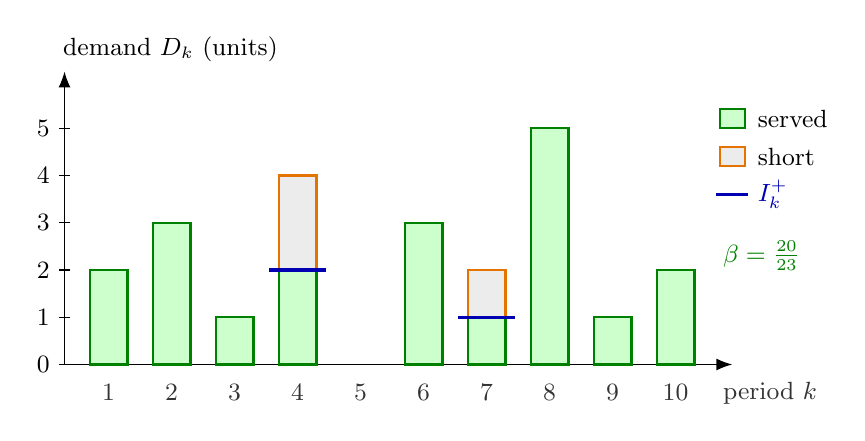
\begin{tikzpicture}[font=\small, >={Latex[length=2mm]}, x=0.8cm, y=0.6cm]
  \draw[->] (0.3,0) -- (10.9,0);
  \draw[->] (0.3,0) -- (0.3,6.2) node[anchor=south west, xshift=-4pt] {demand $D_k$ (units)};
  \foreach \v in {0,1,2,3,4,5} {\draw (0.38,\v) -- (0.22,\v) node[left] {$\v$};}
  % served part
  \foreach \k/\s in {1/2,2/3,3/1,4/2,6/3,7/1,8/5,9/1,10/2}
    {\fill[green!20] (\k-0.3,0) rectangle (\k+0.3,\s); \draw[green!50!black, thick] (\k-0.3,0) rectangle (\k+0.3,\s);}
  % unmet part
  \foreach \k/\s/\d in {4/2/4,7/1/2}
    {\fill[gray!15] (\k-0.3,\s) rectangle (\k+0.3,\d); \draw[orange!90!black, thick] (\k-0.3,\s) rectangle (\k+0.3,\d);}
  % on-hand stock at the start of the short periods
  \foreach \k/\i in {4/2,7/1} {\draw[blue!70!black, very thick] (\k-0.45,\i) -- (\k+0.45,\i);}
  % legend
  \fill[green!20] (10.7,5.0) rectangle (11.1,5.4); \draw[green!50!black, thick] (10.7,5.0) rectangle (11.1,5.4);
  \node[anchor=west] at (11.15,5.2) {served};
  \fill[gray!15] (10.7,4.2) rectangle (11.1,4.6); \draw[orange!90!black, thick] (10.7,4.2) rectangle (11.1,4.6);
  \node[anchor=west] at (11.15,4.4) {short};
  \draw[blue!70!black, very thick] (10.65,3.6) -- (11.15,3.6);
  \node[blue!70!black, anchor=west] at (11.15,3.6) {$I_k^+$};
  \foreach \k in {1,...,10} {\node[gray!40!black] at (\k,-0.6) {$\k$};}
  \node[gray!40!black, anchor=west] at (10.6,-0.6) {period $k$};
  \node[green!50!black, anchor=west] at (10.6,2.3) {$\beta=\frac{20}{23}$};
\end{tikzpicture}
\end{document}
